\RequirePackage[l2tabu, orthodox]{nag} % warns and hints on outdate commands, classes and packages.
% `nag-l2tabu.cfg`: check obsolete packages and commands.
% `nag-orthodox.cfg`: warn about usage that will mostly do unexpected things.

%-----------------------------------------------------------------------------
%	PACKAGES AND DOCUMENT CONFIGURATION
%-----------------------------------------------------------------------------

%% Document class
\documentclass{article}

% If you need to pass options to natbib, use, e.g.:
\bibliographystyle{unsrtnat}
\PassOptionsToPackage{numbers, compress}{natbib}
% before loading neurips_2023

% ready for submission
\usepackage{neurips_2023}

% to compile a preprint version, e.g., for submission to arXiv, add add the
% [preprint] option:
%     \usepackage[preprint]{neurips_2023}

% to compile a camera-ready version, add the [final] option, e.g.:
%     \usepackage[final]{neurips_2023}

% to avoid loading the natbib package, add option nonatbib:
%    \usepackage[nonatbib]{neurips_2023}

% Math packages
\usepackage{amsmath} % AMS math formulas
\usepackage{amssymb} % AMS math symbols (\intercal)
\usepackage{amsfonts} % AMS math fonts: Euler, bb, bf, frak; subscript sizes; Cyrillic
\usepackage{amsopn} % AMS math operators
\DeclareMathOperator{\diag}{diag}
% Use one of the following alternative script fonts:
\usepackage{mathrsfs} % Raph Smith's Formal Script font in mathematics, provides `\mathscr`.
% \usepackage[mathscr]{eucal} % Euler Script, provides `\mathscr`.
% You may force Euler Script to a separate command:
\usepackage{euscript} % Euler Script, provides `\EuScript`.
% Symbol overlapping
\usepackage{mathtools}
% Custom math commands
\renewcommand{\d}{\ensuremath{\mathop{}\!\mathrm{d}}} %differential operator: left space, upright.

% Pseudo-code packages: `algorithmic`, `algorithmicx`, `algorithm2e`.
% see: https://tex.stackexchange.com/q/229355/95794
\usepackage{algorithm} % Float wrapper for algorithms
% Layouts in `algorithmicx`: `algpseudocode`, `algpascal`, `algc`
\usepackage{algpseudocode} % default layout
% \usepackage{algpascal}     % Pascal layout
% \usepackage{algc}          % C layout
\algnewcommand\algorithmicinput{\textbf{Input:}}
\algnewcommand\algorithmicoutput{\textbf{Output:}}
\algnewcommand\algorithmicnote{\textbf{Note:}}
\algnewcommand\Input{\item[\algorithmicinput]}%
\algnewcommand\Output{\item[\algorithmicoutput]}%
\algnewcommand\Note{\item[\algorithmicnote]}%
\def\NoNumber#1{{\def\alglinenumber##1{}\State #1}\addtocounter{ALG@line}{-1}}

%% Tables
\usepackage{threeparttable} %
\usepackage{booktabs}       % professional-quality tables
% \usepackage[skip=0.5\baselineskip]{caption} % Less space blow caption. (Does not work with SIAM)

%% Graphics packages
\usepackage{graphicx} % `graphicx.sty`

% Hypertext marks (back-reference is also desirable.)
\usepackage{hyperref}       % hyperlinks
\usepackage{url}            % simple URL typesetting
\usepackage{xcolor}         % colors

%% Text packages
\usepackage{microtype} % Microtypography, reduce large interword spaces
\usepackage[utf8]{inputenc} % allow utf-8 input
\usepackage[T1]{fontenc}    % use 8-bit T1 fonts
\usepackage[strings]{underscore} % Allow underscore, e.g. in DOIs.
\usepackage[strict=true]{csquotes} % Context sensitive quotation
\usepackage{nicefrac}       % compact symbols for 1/2, etc.
\usepackage{cleveref}       % must be loaded after `hyperref`
\newcommand{\creflastconjunction}{, and~} % Add a serial/Oxford comma by default.
%\crefname{figure}{Fig.}{Figs.} %capitalize and shorten \cref figure labels.
%\Crefname{figure}{Figure}{Figures} %capitalize \Cref figure labels.

% Author comments
\newcommand{\tmp}[1]{\textcolor{white!40!black}{#1}} %temporary text.
\newcommand{\jnk}[1]{\textcolor{white!90!black}{#1}} %junk placeholder text.
\newcommand{\cmtR}[1]{\textcolor{red!50!black}{(Ruda: #1)}} %comment by Ruda.
\newcommand{\RZ}[0]{\textcolor{blue!90!black}{(Ruda)}} %section for Ruda.
\newcommand{\edit}[1]{\textcolor{blue!80!black}{#1}} %New edits.
\newcommand{\todo}[1]{\textcolor{red}{(#1)}}



\title{Bayesian Global Optimization via Rootfinding}

% The \author macro works with any number of authors. There are two commands
% used to separate the names and addresses of multiple authors: \And and \AND.
%
% Using \And between authors leaves it to LaTeX to determine where to break the
% lines. Using \AND forces a line break at that point. So, if LaTeX puts 3 of 4
% authors names on the first line, and the last on the second line, try using
% \AND instead of \And before the third author name.


\author{%
  David S.~Hippocampus\thanks{Use footnote for providing further information
    about author (webpage, alternative address)---\emph{not} for acknowledging
    funding agencies.} \\
  Department of Computer Science\\
  Cranberry-Lemon University\\
  Pittsburgh, PA 15213 \\
  \texttt{hippo@cs.cranberry-lemon.edu} \\
  % examples of more authors
  % \And
  % Coauthor \\
  % Affiliation \\
  % Address \\
  % \texttt{email} \\
  % \AND
  % Coauthor \\
  % Affiliation \\
  % Address \\
  % \texttt{email} \\
  % \And
  % Coauthor \\
  % Affiliation \\
  % Address \\
  % \texttt{email} \\
  % \And
  % Coauthor \\
  % Affiliation \\
  % Address \\
  % \texttt{email} \\
}

\begin{document}


\maketitle


\begin{abstract}
\end{abstract}

\textcolor{red}{TODO:
\begin{itemize}
\item
  Target publication: NeurIPS 2024. (Submission deadline: 2024-05-22 3pm
  CDT.)
\item
  Separate publication: Chebyshev polynomial-based eigenfunctions for BO
  on the hypercube $[-1, 1]^d$, see the Misc section.
\item
  GP hyper-parameter tuning in BO with TS-roots.
\end{itemize}
}

\section{Introduction}

\emph{Optimization problem.} We want to solve the global optimization
problem $\min_{\mathbf{x} \in \mathcal{X}} f(\mathbf{x})$ where the
objective function $f: \mathcal{X} \mapsto \mathbb{R}$ has
$d \in \mathbb{N}_{>0}$ variables taking values in
$\mathcal{X} \subset \mathbb{R}^d$. The objective function
$f(\mathbf{x})$ is costly-to-evaluate so a surrogate-based sequential
optimization approach could work well, and we choose Bayesian
optimization (BO).

At its core, BO approximates the objective function with a stochastic
process such as a Gaussian process (GP), and uses the posterior process
given the current dataset to derive a deterministic surrogate function
that is optimized instead, to find the next design point. If the GP
prior can be represented as a Wiener series where the (adaptive) basis
functions are multivariate polynomials (MVP), the posterior process can
be sampled by truncating the Wiener series and updating the weights, and
each sample is a MVP as well. If we can solve all the critical points of
the sample MVP efficiently, just like solving the roots of a univariate
polynomial as an eigen-decomposition \cite{Trefethen2019}, then we can
estimate the posterior distribution of the global optimal point
$\mathbf{x}_\star|\mathcal{D}$ via Monte Carlo sampling. For example,
Thompson sampling (TS) takes a random sample of
$\mathbf{x}_\star|\mathcal{D}$ and proposes it as the next design
point.

Unfortunately, the problem of solving the distinct roots of an $d$-set
of $d$-variate polynomials is still challenging in general. If the MVP
approximant has some special structure, such as separability or
additivity, then the rootfinding problem can be reduced to univariate
ones, which can be solved using mature algorithms with efficient
implementations.

To enforce such a structure, we explicitly encode it into the model
space. For multivariate stochastic processes, we can enforce
separability, for example, by writing it as a product of univariate
processes, and the structure is maintained in inferring the posterior
process. Of course, the objective function may not have such a
structure, and thus the posterior process fails to converge to it at the
large-sample limit. But in many BO applications, the affordable sample
size is so small (e.g., about a hundred) that it would be hopeless to
find a reasonably accurate approximant in an unstructured function space
unless the design space dimension $d$ is extremely low. By enforcing
some structure, we may break the curse of dimensionality for typical BO
applications.

These are the key ideas of this work.

\section{Background and Related Work}

Thompson sampling.
BoTorch \cite{Balandat2020}.

\section{(Methods)}

Consider a separable Gaussian process prior
$\mathcal{GP}(0, \prod_{i=1}^d \kappa_i)$ such that the eigenvalues
and eigenfunctions $\{(\lambda_{i,j}, \phi_{i,j}(x_i))\}_{j=0}^\infty$
are known analytically for the kernel integral operator of each
univariate kernel $\kappa_i(x_i, x_i')$ with respect to some
probability measure $\mu_i$ on $\mathbb{R}$. Moreover, we assume
that the eigenfunctions have the form
$\phi_{i,j}(x_i) = p_{i,j}(x_i) \exp(q_i(x_i))$ where $p_{i,j}$ and
$q_i$ are polynomials. These assumptions are satisfied by the default
kernel choice in BO: the separable squared exponential (SE) kernel, also
known as the automatic relevance determination (ARD) kernel. The
eigenfunctions of the SE kernel, with respect to the standard Gaussian
measure, are Hermite polynomials weighted by a common Gaussian function,
see Supplemental Materials.

Our main algorithm is outlined in \cref{alg:TS-roots}.

% Algorithm: TS-roots
\alglanguage{pseudocode}
\begin{algorithm}[h]
  \caption{\texttt{TS-roots}: Global optimization of a separable % posterior
    Thompson sample via rootfinding.}
  \label{alg:TS-roots}
  \begin{algorithmic}[1] % 0, no line numbering; 1, number every line; n, number every n lines.
    \Input eigenpairs
    $\mathcal{S} = \{(\lambda_{i,j}, \phi_{i,j}(x_i) = p_{i,j}(x_i) \exp(q_i(x_i)))\}_{i \in d}^{j \in N_i}$,
    dataset $\mathcal{D}$,
    \edit{stopping criterion $\delta$}
    \State sample prior weights: $\mathbf{w} = (w_{i,j})_{i \in d}^{j \in N_i}$,
    $w_{i,j} \overset{\text{iid}}{\sim} \mathcal{N}0, 1)$.
    \State find minimum-change solution to data constraints:
    $\mathbf{w} \gets \texttt{newton}(\mathbf{w}, \mathcal{S}, \mathcal{D}, \edit{\delta})$
    \State univariate global rootfinding: $\{x_{i,k}\}_{k=1}^{r_i} \gets \mathrm{roots}(p_i(x_i))$,
    $i \in \{1, \cdots, d\}$, where \newline
    $p_i(x_i) = \sum_{j=0}^{N_i - 1} w_{i,j} \sqrt{\lambda_{i,j}} (p_{i,j}(x_i) q'_i(x_i) + p'_{i,j}(x_i))$
    \State evaluate $\{f_{i,k} = f_i(x_{i,k}; \mathbf{w}_i)\}_{i \in d}^{k \in r_i}$, where
    $f_i(x_i; \mathbf{w}_i) = \sum_{j=0}^{N_i - 1} w_{i,j} \sqrt{\lambda_{i,j}} \phi_{i,j}(x_i)$
    \State $(\mathbf{x}^\bot, \mathbf{x}^\top, f^\bot, f^\top) \gets
    \mathrm{sepopt}(x_{i,k}, f_{i,k})_{i \in d}^{k \in r_i}$
    \Output $\mathbf{x}^\bot$
    % \Note 
  \end{algorithmic}
\end{algorithm}

NOTE: \Cref{alg:newton} is a fast approximate approach to sampling the posterior
weights $\mathbf{w} | \mathcal{D}$. Considering that Thompson sampling
is a heuristic approach to balancing the exploitation--exploration
trade-off in BO, it is unnecessary to sample the posterior exactly. If
exact sampling or a truly Bayesian approach is desirable, one may use a
Gibbs sampler instead. \cmtR{Consult Yabo.}

% Algorithm: newton
\alglanguage{pseudocode}
\begin{algorithm}[h]
  \caption{\texttt{newton}: Approximate spectral sampling
    of a separable posterior stochastic process.}
  \label{alg:newton}
  \begin{algorithmic}[1] % 0, no line numbering; 1, number every line; n, number every n lines.
    \Input prior weights: $\mathbf{w}$, eigenpairs $\mathcal{S}$,
    dataset $\mathcal{D}$, stopping criterion $\delta$
    \State $\mathbf{f} \gets (f(\mathbf{x}^k; \mathbf{w}))_{k=1}^n$, where
    $f(\mathbf{x}; \mathbf{w}) = \prod_{i=1}^d f_i(x_i; \mathbf{w}_i)$
    \While{$|\mathbf{y} - \mathbf{f}| < \delta$}
      \State $\mathbf{J} \gets (\nabla_{\mathbf{w}} f(\mathbf{x}^k; \mathbf{w}))_{k \in n}
      \in \mathbb{R}^{n \times N}$, where $J_{k,(j,i)} =
      {f(\mathbf{x}^k; \mathbf{w})} \sqrt{\lambda_{i,j}} \phi_{i,j}(x_i^k) / {f_i(x_i^k; \mathbf{w}_i)}$
      \State $\mathbf{w} \gets \mathbf{w} - \mathbf{J}^\dagger (\mathbf{f} - \mathbf{y})$
      \State $\mathbf{f} \gets (f(\mathbf{x}^k; \mathbf{w}))_{k=1}^n$
    \EndWhile
    \Output $\mathbf{w}$
  \end{algorithmic}
\end{algorithm}

\begin{figure}[t]
  \centering
  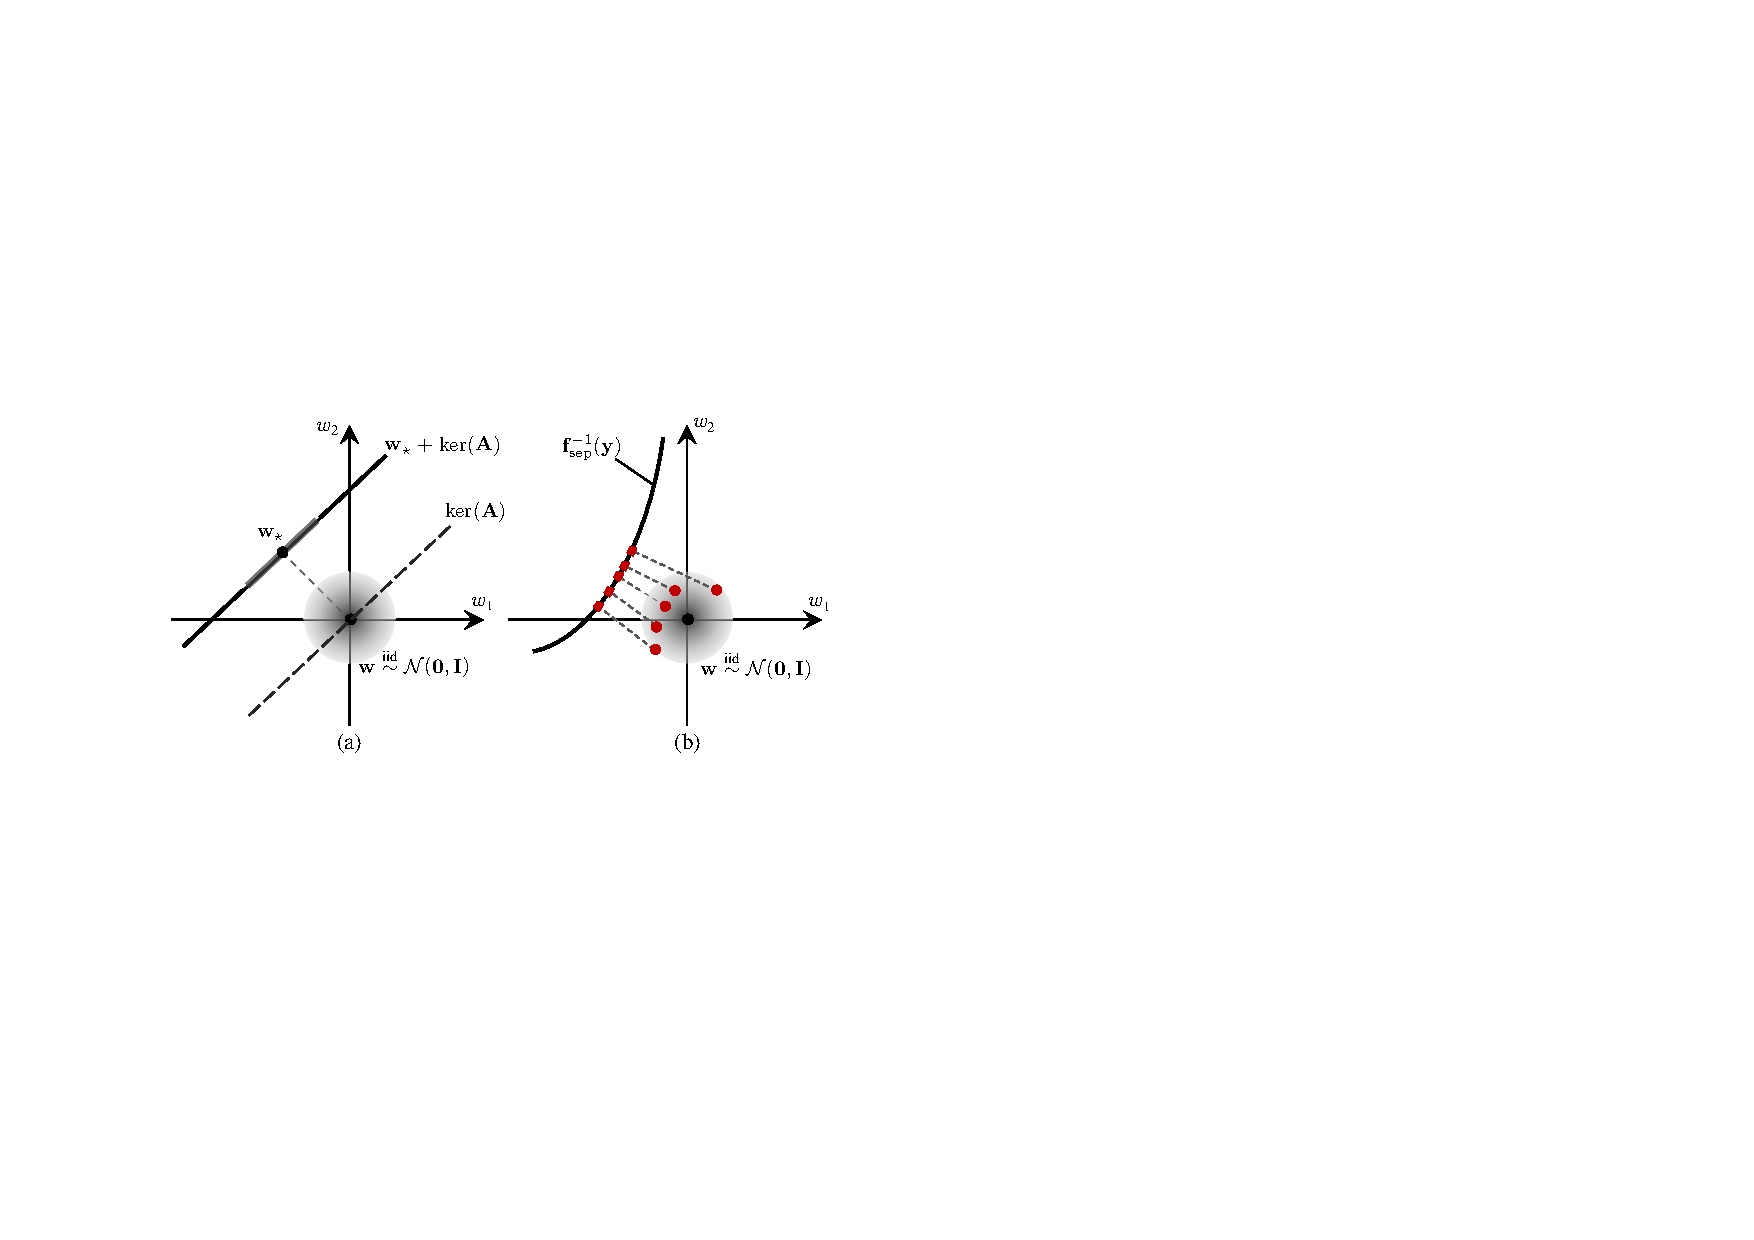
\includegraphics[width=0.75\linewidth]{img/projection.pdf}
  \caption{Spectral sampling for the posterior process.
    (a) Roots of the linear equations $\mathbf{f}(\mathbf{w}) := \mathbf{A} \mathbf{w} = \mathbf{y}$
    form an affine subspace $\mathbf{w}_\star + \ker(\mathbf{A})$,
    and the posterior distribution is equivalent to the orthogonal projection onto the subspace.
    (b) Roots of the nonlinear equations $\mathbf{f}_{\mathrm{sep}}(\mathbf{w}) :=
    \odot_{i=1}^d \mathbf{A}_i \mathbf{w}_i = \mathbf{y}$, where $\odot$ denotes the Hadamard product,
    form a nonlinear manifold $\mathbf{f}_{\mathrm{sep}}^{-1}(\mathbf{y})$.
    The posterior distribution is the prior distribution restricted to the manifold,
    and can be approximately sampled via projection by minimizing distance.}
  \label{fig:projection}
\end{figure}


The critical points of a separable multivariate function are exactly the
The critical points of a \edit{completely multiplicatively} separable multivariate function are exactly the
critical points of its univariate components, arbitrarily combined,
except for when the function value is zero. We ignore the roots of the
function as uninteresting for the optimization problem. Therefore, we
can find all the relevant critical points by solving a global
rootfinding problem for the derivative of each univariate component:
$f_i'(x_i) = 0$, $i \in \{1, \cdots, d\}$. (Proof is simple and
omitted for the moment.)

Solving all roots of a univariate function can be done very efficiently
via Chebyshev/Legendre polynomial approximation and solving an
eigenvalue problem, see e.g., ATAP \cite{Trefethen2019}. The procedure
is outlined in \cref{alg:roots}.

% Algorithm: roots
\alglanguage{pseudocode}
\begin{algorithm}[h]
  \caption{\texttt{roots}: Univariate global rootfinding on an interval.}
  \label{alg:roots}
  \begin{algorithmic}[1] % 0, no line numbering; 1, number every line; n, number every n lines.
    \Input polynomial $p(x)$ of degree $n$ (or any function $f(x)$)
    \State transform into (or approximate in) a Chebyshev/Legendre polynomial basis\newline
    $p(x) = \sum_{k=0}^n a_k T_k(x)$, e.g., via Chebyshev/Legendre interpolation.
    \State solve all the eigenvalues of the colleague/comrade matrix:\newline
    the colleague matrix can be written as
    $C = [\mathrm{band}((-1, 1), 1) + [1]_{1,2} - (a_{-n} / a_n)_{n,}] / 2$
    \Output all the real eigenvalues $\{x_i\}_{i=1}^r$ in the interval
  \end{algorithmic}
\end{algorithm}

NOTE: For a sample from a univariate GP with an SE kernel, generated by
truncating the Wiener series to $N+1$ terms, its critical points are
the roots of a degree-$(N+1)$ Hermite polynomial series (on
$\mathbb{R}$).

NOTE: Efficient algorithms for the global rootfinding in Chebyshev basis
have been implemented in the Chebfun package in MATLAB [Battles and
Trefethen, 2005], which also implements Chebfun
interpolation. Any software implementation in R or Python?

NOTE: If we use Chebyshev/Legendre interpolation,
then \cref{alg:roots} can be applied to any spectral representation of a stochastic process.
For representations in the Fourier basis
(e.g., Matern-like kernels and Bochner's representation of stationary kernels),
evaluation of the posterior sample can be done efficiently using the fast Fourier transform,
in $\mathcal{O}(N_i \log N_i)$ flops.

\todo{TODO: fast evaluation of Hermite polynomial series; Chebyshev
interpolation; global rootfinding of a Chebyshev polynomial.}

Given all the critical points and values of the univariate components,
computing the global optimal points and values of a separable function
does not require computing all the combinations of the component
critical values. An efficient approach is given in \cref{alg:sepopt}. (Proof is
simple and we omit it here.)

% Algorithm: sepopt
\alglanguage{pseudocode}
\begin{algorithm}[h]
  \caption{\texttt{sepopt}: Global optimization of a separable function.}
  \label{alg:sepopt}
  \begin{algorithmic}[1] % 0, no line numbering; 1, number every line; n, number every n lines.
    \Input component critical points and values $(x_{i,j}, f_{i,j})_{i \in d}^{j \in r_i}$
    \State $(i, j^\top_{\mathrm{abs}}) \gets \arg\max_{j \in r_i} |f_{i,j}|$, $i \in d$
    \State $\mathbf{x}_{\mathrm{abs}}^\top \gets (x_{i, j^\top_{\mathrm{abs}}})_{i=1}^d$
    \State $f_{\mathrm{abs}}^\top \gets \prod_{i=1}^d f_{i, j^\top_{\mathrm{abs}}}$
    \State $r_{i,j} \gets f_{i,j} / f_{i, j^\top_{\mathrm{abs}}}$
    \State $(i, j^\bot_{\mathrm{rel}}) \gets \arg\min_{j \in r_i} r_{i,j}, i \in d$
    \If{$\min_{i \in d} r_{i, j^\bot_{\mathrm{rel}}} \ge 0$}
    \State $\mathbf{x}_{\mathrm{alt}}^\bot \gets (x_{i, j^\bot_{\mathrm{rel}}})_{i=1}^d$
    \State $f_{\mathrm{alt}}^\bot \gets \prod_{i=1}^d f_{i, j^\bot_{\mathrm{rel}}}$
    \Else
    \State $i' \gets \arg\min_{i \in d} r_{i, j^\bot_{\mathrm{rel}}}$
    \State $\mathbf{x}_{\mathrm{alt}}^\bot \gets (x_{1, j^\top_{\mathrm{abs}}}, \cdots,
    x_{i', j^\bot_{\mathrm{rel}}}, \cdots, x_{d, j^\top_{\mathrm{abs}}})$
    \State $f_{\mathrm{alt}}^\bot \gets (\prod_{i \ne i'} f_{i, j^\top_{\mathrm{abs}}})
    f_{i', j^\bot_{\mathrm{rel}}}$
    \EndIf
    \If{$f_{\mathrm{abs}}^\top > 0$}
    \State \Return $(\mathbf{x}_{\mathrm{alt}}^\bot, \mathbf{x}_{\mathrm{abs}}^\top,
    f_{\mathrm{alt}}^\bot, f_{\mathrm{abs}}^\top)$
    \Else
    \State \Return $(\mathbf{x}_{\mathrm{abs}}^\top, \mathbf{x}_{\mathrm{alt}}^\bot,
    f_{\mathrm{abs}}^\top, f_{\mathrm{alt}}^\bot)$
    \EndIf
    \Note The output, understood as $(\mathbf{x}^\bot, \mathbf{x}^\top, f^\bot, f^\top)$,
  are the global minimal and maximal points and the global minimum and maximum, respectively.
  \end{algorithmic}
\end{algorithm}


\section{Experiments}

\section{Discussion}

\subsection{Broader Impact}


\section{Supplementary Material}

\subsection{Bayesian Optimization via Spectral Sampling}

A general procedure for sequential optimization is given in Alg A.1; see
\cite{Garnett2023} Alg 1.1. The initial dataset can either be empty or
contain some pairs of inputs and observations; in the latter case we can
write $\mathcal{D}^0 = \{(\mathbf{x}^i, y^i)\}_{i=1-n_0}^0$, where
$n_0 \in \mathbb{N}_{>0}$. Three components of this algorithm can be
customized: the observation model $\mathrm{Observe}(\mathbf{x})$, the
termination condition, and the optimization policy
$\mathrm{Policy}(\mathcal{D})$.

% Algorithm: sequential optimization 
\alglanguage{pseudocode}
\begin{algorithm}[h]
  \caption{Sequential optimization \cite{Garnett2023}.}
  \label{alg:seqopt}
  \begin{algorithmic}[1] % 0, no line numbering; 1, number every line; n, number every n lines.
    \Input initial dataset $\mathcal{D}^0$
    \State $k \gets 1$
     \Repeat
      \State $\mathbf{x}^k \gets \mathrm{Policy}(\mathcal{D}^{k-1})$
      \State $y^k \gets \mathrm{Observe}(\mathbf{x}^k)$ 
      \State $\mathcal{D}^k \gets \mathcal{D}^{k-1} \cup \{(\mathbf{x}^k, y^k)\}$
    \Until{termination condition reached}
    \Output  $\mathcal{D}$
  \end{algorithmic}
\end{algorithm}

Bayesian optimization (BO) is can be seen as an optimization policy for
sequential optimization; a formal procedure is given in Alg A.2. Three
components of this algorithm can be customized: the prior probabilistic
model $\widehat{f}^0$, the acquisition function
$\alpha(\mathbf{x})$, and the global optimization algorithm. Any
probabilistic model $\widehat{f}$ of the objective function $f$ can
be seen as a probability distribution on a function space, and the prior
$\widehat{f}^0$ is usually specified as a stochastic process such as a
Gaussian process (GP). The acquisition function $\alpha(\mathbf{x})$
derived from $\widehat{f}$ can be either deterministic (such as the
Expected Improvement) or stochastic (such as Thompson Sampling). Note
that to simplify notation, we stated the global optimization problem of
$\alpha(\mathbf{x})$ as minimization rather than maximization; the two
problems are exactly the same with a change of sign to the objective.

% Algorithm: Bayesian optimization policy
\alglanguage{pseudocode}
\begin{algorithm}[h]
  \caption{Bayesian optimization policy.}
  \label{alg:BOpolicy}
  \begin{algorithmic}[1] % 0, no line numbering; 1, number every line; n, number every n lines.
    \Input a prior stochastic process $\widehat{f}^0$ for the objective function $f$, current dataset $\mathcal{D}^{k-1}$
    \State determine posterior
    $\widehat{f}^k := \widehat{f}^0 | \mathcal{D}^{k-1}$
    \State derive acquisition function $\alpha^k(\mathbf{x})$ from
    $\widehat{f}^k$
    \State $\mathbf{x}^k \gets \arg\min_{\mathbf{x} \in \mathcal{X}} \alpha^k(\mathbf{x})$
    \State \Return $\mathbf{x}^k$
  \end{algorithmic}
\end{algorithm}

When applied to BO, Thompson sampling (TS) generates a random
acquisition function simply by sampling the posterior model. The
procedure is formalized in Alg A.3.

% Algorithm: Bayesian optimization policy
\alglanguage{pseudocode}
\begin{algorithm}[h]
  \caption{Thompson sampling acquisition function.}
  \label{alg:TS}
  \begin{algorithmic}[1] % 0, no line numbering; 1, number every line; n, number every n lines.
    \Input posterior $\widehat{f}^k$
    \State \Return $\alpha^k(\mathbf{x}) \sim \widehat{f}^k$
  \end{algorithmic}
\end{algorithm}

We can sample a Gaussian process $\mathcal{GP}(m, \kappa)$
efficiently, if we have a spectral representation of the covariance
function $\kappa(\mathbf{x}, \mathbf{x}')$ that converges quickly. By
spectral representation, we mean a series of rank-one kernels (aka
positive type functions). Per the Mercer's theorem on probability spaces
(see e.g., \cite{Rasmussen2006} Sec 4.3), any kernel that is
essentially bounded with respect to some probability measure $\mu$ on
the domain $\mathcal{X}$ has a spectral representation
$\kappa(\mathbf{x}, \mathbf{x}') = \sum_{i=0}^\infty \lambda_i \phi_i(\mathbf{x}) \phi_i(\mathbf{x}')$,
where $(\lambda_i, \phi_i(\mathbf{x}))$ is a pair of eigenvalue and
eigenfunction of the kernel integral operator $T_\kappa$ and the
eigenvalues are sorted in decreasing order such that
$\lambda_i \ge \lambda_{i+1} \ge 0$, $i \in \mathbb{N}$. The kernel
integral operator is defined by its action on a function as
$(T_\kappa f)(\mathbf{x}) := \int_{\mathcal{X}} \kappa(\mathbf{x}, \mathbf{x}') f(\mathbf{x}') \mu(d \mathbf{x}')$.
The eigenfunctions satisfy $T_\kappa \phi_i = \lambda_i \phi_i$ and
they are orthonormal in $L^2_\mu(\mathcal{X})$. The covariance
functions of GP priors commonly used in Bayesian optimization usually
have a spectral representation known in analytical form. Suppose this is
the case, we can sample the GP prior as a truncated Wiener series, see
Alg A.4.

% Algorithm: unconditional spectral sampling
\alglanguage{pseudocode}
\begin{algorithm}[h]
  \caption{Spectral sampling of Gaussian process prior.}
  \label{alg:sam_priorGP}
  \begin{algorithmic}[1] % 0, no line numbering; 1, number every line; n, number every n lines.
    \Input mean function $m(\mathbf{x})$, eigenpairs
  $\{(\lambda_i, \phi_i(\mathbf{x}))\}_{i=0}^{N-1}$
    \State $w_i \overset{\text{iid}}{\sim} \mathcal{N}(0,1)$
    \State \Return $f(\mathbf{x}) \gets m(\mathbf{x}) + \sum_{i=0}^{N-1} w_i \sqrt{\lambda_i} \phi_i(\mathbf{x})$
  \end{algorithmic}
\end{algorithm}

To simplify notation, we assume that the GP prior mean function
$m(\mathbf{x}) = 0$. If the observation model
$\mathrm{Observe}(\mathbf{x})$ can be written as
$y^i = f(\mathbf{x}^i) + z^i$ where
$z^i \overset{\text{iid}}{\sim} \mathcal{N}(0, \varepsilon^2)$, then the
posterior given dataset
$\mathcal{D} = \{(\mathbf{x}^i, y^i)\}_{i=1}^n$ is also a Gaussian
process
$\widehat{f}^0 | \mathcal{D} \sim \mathcal{GP}(m_{\mathcal{D}}, \kappa_{\mathcal{D}})$,
where
$m_{\mathcal{D}}(\mathbf{x}) = \mathbf{y}^\intercal (\mathbf{K} + \varepsilon^2 \mathbf{I}_n)^{-1} \mathbf{k}(\mathbf{x})$
and
$\kappa_{\mathcal{D}}(\mathbf{x}, \mathbf{x}') = \kappa(\mathbf{x}, \mathbf{x}') - \mathbf{k}(\mathbf{x})^\intercal (\mathbf{K} + \varepsilon^2 \mathbf{I}_n)^{-1} \mathbf{k}(\mathbf{x}')$.
Here we denote
$\mathbf{K} = [\kappa(\mathbf{x}^i, \mathbf{x}^j)]_{i \in n}^{j \in n}$
and
$\mathbf{k}(\mathbf{x}) = (\kappa(\mathbf{x}, \mathbf{x}^i))_{i=1}^n$.

The GP posterior can be sampled as an updated truncated Wiener series
$\widehat{f}^0 | \mathcal{D} = \sum_{k=0}^{N-1} \widetilde{w}_k \sqrt{\lambda_k} \phi_k(\mathbf{x})$,
where
$\widetilde{\mathbf{w}} \sim \mathcal{N}_N(\mathbf{w}_\star, \boldsymbol{\Sigma}_\star)$.
Let $\boldsymbol{\Phi} = [\phi_j(\mathbf{x}^i)]_{i \in n}^{j \in N}$,
$\boldsymbol{\Lambda} = \mathrm{diag}(\lambda_i)_{i \in N}$ and
$\mathbf{A} = \boldsymbol{\Phi} \boldsymbol{\Lambda}^{1/2}$. Assume
that the observation is noiseless (i.e., $\varepsilon = 0$), we have
the posterior mean $\mathbf{w}_\star = \mathbf{A}^\dagger \mathbf{y}$
and the posterior covariance
$\boldsymbol{\Sigma}_\star = \mathbf{P}_{\ker(\mathbf{A})}$. Here
$\dagger$ denotes the Moore--Penrose inverse, $\ker()$ denotes the
kernel (or null space) of a matrix, and $\mathbf{P}$ denotes the
orthogonal projection operator onto a subspace. Assume that
$\mathrm{rank}(\mathbf{A}) = n < N$ and let
$\mathbf{A} = \mathbf{U} \mathbf{D} \mathbf{V}^\intercal$ be a thin
SVD, we have
$\mathbf{A}^\dagger = \mathbf{A}^\intercal (\mathbf{A} \mathbf{A}^\intercal)^{-1}$
and
$\mathbf{P}_{\ker(\mathbf{A})} = \mathbf{I}_N - \mathbf{V} \mathbf{V}^\intercal$.

\emph{Spectral sampling of Gaussian process posterior is equivalent to
projection, given noiseless observations.} From Alg A.4 we see that the
prior weights $\mathbf{w} = (w_i)_{i=1}^N$ is a standard Gaussian
random vector. With noiseless observations, the posterior weights
$\widetilde{\mathbf{w}}$ is distributed as the prior distribution
restricted to set of points satisfying
$\mathbf{f}(\mathbf{w}) = \mathbf{y}$, where
$\mathbf{f}(\mathbf{w}) := (f(\mathbf{x}^i; \mathbf{w}))_{i=1}^n$ with
$f(\mathbf{x}; \mathbf{w}) = \sum_{i=0}^{N-1} w_i \sqrt{\lambda_i} \phi_i(\mathbf{x})$.
This set---the preimage $\mathbf{f}^{-1}(\mathbf{y})$---is the affine
subspace $\mathcal{S} = \mathbf{w}_\star + \ker(\mathbf{A})$. For a
multivariate Gaussian distribution, its restriction to an affine
subspace is the same with its orthogonal projection onto the subspace;
and therefore
$\widetilde{\mathbf{w}} \sim \mathbf{w}|_{\mathcal{S}} \sim \mathbf{P}_{\mathcal{S}} \mathbf{w}$.
This allows us to sample the GP posterior via projection, see Alg A.5.

% Algorithm: conditional spectral sampling
\alglanguage{pseudocode}
\begin{algorithm}[h]
  \caption{Spectral sampling of Gaussian process posterior.}
  \label{alg:sam_postGP}
  \begin{algorithmic}[1] % 0, no line numbering; 1, number every line; n, number every n lines.
    \Input eigenpairs $\{(\lambda_i, \phi_i(\mathbf{x}))\}_{i=0}^{N-1}$,
  dataset $\mathcal{D}$
    \State $\mathbf{w} \gets (w_i)_{i=0}^{N-1}$, where
  $w_i \overset{\text{iid}}{\sim} \mathcal{N}(0,1)$
    \State $\mathbf{A} \gets [\lambda_j \phi_j(\mathbf{x}^i)]_{i \in n}^{j \in N}$
    \State $\mathbf{A} = \mathbf{U} \mathbf{D} \mathbf{V}^\intercal$ \Comment{thin SVD}
    \State $\mathbf{w}_\star \gets \mathbf{V} \mathbf{D}^\dagger \mathbf{U}^\intercal \mathbf{y}$
    \State $\widetilde{\mathbf{w}} \gets \mathbf{w}_\star + \mathbf{w} - \mathbf{V} \mathbf{V}^\intercal \mathbf{w}$
    \State \Return $f(\mathbf{x}) \gets \sum_{i=0}^{N-1} \widetilde{w}_i \sqrt{\lambda_i} \phi_i(\mathbf{x})$
  \end{algorithmic}
\end{algorithm}

\subsection{Spectrum of the SE Kernel}

\edit{
The univariate squared exponential (SE) kernel can be written as
$k(x, x'; \rho) = \exp(-\frac{\rho}{1-\rho} s^2)$, where relative distance $s = |x - x'|$ and $\rho \in (0,1)$.
The length scale $l$ relates to $\rho$ via $\frac{1}{2 l^2} = \frac{\rho}{1-\rho}$.
Mehler's formula allows us to determine the eigenvalues and eigenfunctions of the kernel integral operator as follows \cite{Vinaroz2022}:
% 
\begin{equation}\label{}
	\exp(-\frac{\rho}{1-\rho} (x - x')^2) = \sum_{k=0}^{\infty} \lambda_k \phi_k(x) \phi_k(x').
\end{equation} 
For $k \in \mathbb{N}$, the $k$th eigenvalue and the corresponding eigenfunction are $\lambda_k = (1-\rho) \rho^k$ and
$\phi_k(x) = \frac{1}{\sqrt{N_k}} \exp\left(-\frac{\rho}{1+\rho} x^2\right) H_k(x)$, where $N_k = 2^c c! \sqrt{\frac{1-\rho}{1+\rho}}$ and $H_k(x)$ the $k$th-order Hermite polynomial defined by
$H_k(x) = (-1)^k \exp(x^2) \frac{d^k}{dx^k} \exp(-x^2)$.
This result can also be derived from Mercer's theorem, as outlined in \cite{ZhuHY1998}.
}

%The univariate squared exponential (SE) kernel can be written as
%$k(x, x'; l) = \exp(-\frac{1}{2} s^2)$, where relative distance $s = |x - x'| / l$.
%With a Gaussian measure $\mu = \mathcal{N}(0, \sigma^2)$ over the domain $X = \mathbb{R}$,
%we can write the eigenvalues and eigenfunctions of the kernel integral operator as follows.
%(See e.g., \cite{ZhuHY1998} Sec. 4 and \cite{Gradshteyn2014} 7.374 eq. 8.)
%
%Denote normalized coordinate $x_\sigma = x / \sigma$ and normalized lengthscale $l_\sigma = l / \sigma$.
%Define constants $\alpha = (\frac{1}{4} + l_\sigma^{-2})^{\frac{1}{4}} > 2^{-\frac{1}{2}}$ and
%$\beta = \frac{1}{2} l_\sigma^2 + 1 + (\frac{1}{4} l_\sigma^4 + l_\sigma^2)^{\frac{1}{2}} > 1$.
%For $k \in \mathbb{N}$, the $k$th eigenvalue is $\lambda_k = l_\sigma \beta^{-\frac{1}{2} - k}$,
%and a corresponding eigenfunction is
%$\phi_k(x) = \exp\{-\frac{1}{2}(\alpha^2 - \frac{1}{2}) x_\sigma^2\} \cdot H_k(\alpha x_\sigma)$,
%where $H_k(x)$ is the $k$th-order Hermite polynomial defined by
%$H_k(x) := (-1)^k \exp(x^2) \frac{d^k}{dx^k} \exp(-x^2)$.

\section{Misc: Chebyshev Polynomial-based Spectral Representation
  for BO on the Hypercube}

\textcolor{red}{TODO:
\begin{itemize}
\item
  Feedback collection: NeurIPS 2024 workshops, 2024-12-14:15.
  (Submission deadline: 2024-09-26 or soon after.)
\item
  Target publication: TBD (ICML 2025, paper due late Jan 2025; previous
  due dates: 2024-02-01, 2023-01-26, 2022-01-27, 2021-02-04,
  2020-02-06).
\end{itemize}
}



\section*{References}

\bibliography{TS-roots}

\end{document}
